\documentclass{article}
\usepackage{algorithm}
\usepackage{algpseudocodex}
\usepackage{graphicx}
\usepackage{amsmath}
\title{CSEP521 : Applied Algorithms: Midterm}
\author{Karuna Sagar Krishna}

\begin{document}
    \maketitle

    \section*{Question 1}

    \subsection*{1a}
    \textbf{False}

    If $n^{3.05} = O(n^3 \log n)$ is true, then
    
    \begin{align*}
        n^{3.05} & <= c(n^3 \log n) && \text{by definition of O, for some $c > 0$ and $n > n_0$} \\
        n^{3+0.05} & <= c n^3 \log n \\
        n^3 n^{0.05} & <= c n^3 \log n \\
        n^{0.05} & <= c \log n && \text{this contradicts $\log n = O(n^x) : x > 0$ as seen in class} \\
    \end{align*}

    Hence, $n^{3.05} = O(n^3 \log n)$ is \textbf{false}.

    \subsection*{1b}
    \textbf{False}
    
    If $2^n = \Omega(2^{2n})$ is true, then
    
    \begin{align*}
        2^n & >= c(2^{2n}) && \text{by definition of $\Omega$, for some $c > 0$ and $n > n_0$} \\
        1 & >= c2^n && \text{divide both sides by $2^n$} \\
          &         && \text{since $c > 0$ and $n > n_0$, this is a contradiction}
    \end{align*}

    Hence, $2^n = \Omega(2^{2n})$ is \textbf{false}.

    \subsection*{1c}
    \textbf{True}
    
    Breadth first search algorithm runs in $O(n+m)$ time (polynomial time) and can decide if the graph has odd length cycle or not. We used this in class to verify if a graph is 2-colorable or bipartite since bipartite graphs cannot contain odd length cycles.

    \subsection*{1d}
    \textbf{False}

    Let's say $T(n) = 3T(n/2) + n^5$ so that we can apply master recurrence theorem with $a = 3, b = 2, c = 1, d = 5$. Clearly, $a < b^d$ since $3 < 2^5$ hence $T(n) = \Theta(n^5)$. But we are given $T(n) <= 3T(n/2) + n^5$, so $T(n) = O(n^5)$. So, $T(n) = O(n^3)$ is \textbf{false}.

    \subsection*{1e}
    \textbf{False}

    Consider a circular graph with all edges having the same weight $w$ (no distinct weights). The MST for this graph would have to include all edges except one, if not the spanning tree is not connected. So it cannot exclude both/all of the heavy edges.

    \subsection*{1f}
    \textbf{True}

    The cut property of MST says that the minimum weight edge crossing any cut must be included in every MST. Consider a cut formed by $\{v\}$ and $V-\{v\}$, clearly, $e$ is the minimum weight edge crossing this cut and by cut property $e$ should be included in every MST.
    
    Further, if we apply cut property repeatedly on each vertex in $G$, then the unique lightest edge touching each vertex should be included in every MST.

    \subsection*{1g}
    \textbf{True}

    From class, the best known algorithm for multiplying two n-bit integers runs in $\Theta(n \log(n) \log(\log n))$. Let's compare $O(n^{1.1})$ and $\Theta(n \log(n) \log(\log n))$. Note, $\Theta$ is both $O$ and $\Omega$ at the same time, so let's specifically compare $O(n^{1.1})$ and $O(n \log(n) \log(\log n))$.

    \begin{align*}
        f(n) & = O(n^{1.1}) \\
        f(n) & <= c_0(n^{1.1}) && \text{for some $c_0 > 0$ and $n > n_0$} \\
        (1/n)f(n) & <= c_0 n^{0.1} \\
        \\
        g(n) & = O(n \log(n) \log(\log n)) \\
        g(n) & <= c_1(n \log(n) \log(\log n)) && \text{for some $c_1 > 0$ and $n > n_1$} \\
        (1/n)g(n) & <= c_1 \log(n) \log(\log n)
    \end{align*}

    As we learnt in class that \textit{log grows slower than every polynomial}, we can conclude that $c_1 \log(n) \log(\log n)$ grows slower than $c_0 n^{0.1}$. Hence, $(1/n)g(n)$ grows slower than $(1/n)f(n)$, which implies $O(n \log(n) \log(\log n))$ grows slower than $O(n^{1.1})$. So, the best known algorithm is upper bounded by $O(n^{1.1})$.

    \subsection*{1h}
    \textbf{False}

    The matching of size $k$ contains $k$ edges that don't touch each other. So the graph $G$ has atleast $k$ disjoint edges. Any vertex cover should cover these $k$ disjoint edges. Since the $k$ edges are disjoint, we need to include atleast one vertex touching each of the edge i.e. vertex cover should contain atleast $k$ vertices. If there is a vertex cover of size $k-1$, then by pigeon hole principle there must be a vertex that is covering more than one of these $k$ disjoint edges which is not possible because there are no two edges which share a vertex. Hence vertex cover of size $k-1$ is not possible.

    \subsection*{1i}
    \textbf{False}

    Assuming that the statement given is true then there is a polynomial time algorithm to determine if atmost $\sqrt n$ sets can cover the whole universe. This is a specific version of the set cover decision problem - can atmost $k$ sets cover the whole universe which is known to be NP-complete. Given this our assumption must be false i.e. there is no polynomial time algorithm to determine if atmost $\sqrt n$ sets can cover the whole universe.

    \section*{Question 2}

    \subsection*{Idea}
    The question indicates that cells are labelled as $x$, $y$, etc. To clarify, each cell in the checkerboard is labelled with an integer as follows - label the bottom left cell with 1, proceed labelling the adjacent right cell incrementing the label and then repeating for the next row on the top.

    \begin{figure}[H]
        \begin{center}
            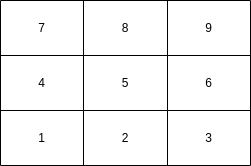
\includegraphics[width=0.35\textwidth]{checkerboard.png}
        \end{center}
    \end{figure}

    The goal is to find the maximum points that can be earned by starting at some cell in bottom row and ending at some cell in the top row. And at each step we have 3 options to move. Intuitively, we could explore all the options and find the maximum. However, this can lead to lot of repetitions. To avoid that we can think of computing the maximum points that can be earned ending at particular cell from some starting cell in bottom row i.e. $maxPointsAt(x)$. To compute this, we notice that a cell can only be reached from previous row and there only 3 cells in this previous row that can be used, specifically a cell $x$ can be reached from cells: $x-n$, $x-n-1$ and $x-n+1$. We can then answer the question by finding the maximum over all the cells in the top row.

    \begin{equation*}
        maxPointsAt(x) = 0 : x \in \{ 1 \dots n \}
    \end{equation*}

    \begin{equation*}
        \begin{split}
            maxPointsAt(x) = 
            max \biggl(
                & maxPointsAt(x-n) + p(x-n, x), \\
                & maxPointsAt(x-n-1) + p(x-n-1, x), \\
                & maxPointsAt(x-n+1) + p(x-n+1, x) \biggr)
        \end{split}
    \end{equation*}

    \begin{equation*}
        maxPoints() = max(maxPointsAt(x)) : x \in \{ n^2 \dots n^2-n+1 \}
    \end{equation*}

    \subsection*{Algorithm}
        \begin{algorithm}[H]
            \begin{algorithmic}
                \Procedure{MaxPoints}{$p$}
                    \For{$i \in \{ 1 \dots n \}$}
                        \State $maxPointsAt[i] = 0$
                    \EndFor

                    \For{$i \in \{ n+1 \dots n^2 \}$}
                        \State $option1 = maxPointsAt[i-n] + p(i-n, i)$
                        \If{$i \mod n \ne 1$}
                            \State $option2 = maxPointsAt[i-n-1] + p(i-n-1, i)$
                        \EndIf
                        \If{$i \mod n \ne 0$}
                            \State $option3 = maxPointsAt[i-n+1] + p(i-n+1, i)$
                        \EndIf
                        \State $maxPointsAt[i] = max(option1, option2, option3)$
                    \EndFor

                    \For{$i \in \{ n^2-n+1 \dots n^2 \}$}
                        \State $maxPoints = max(maxPoints, maxPointsAt[i])$
                    \EndFor

                    \State \Return $maxPoints$
                \EndProcedure
            \end{algorithmic}
        \end{algorithm}

    \subsection*{Correctness}
    Let's prove $maxPointsAt$ is correct. For cells in bottom row, $maxPointsAt[i] = 0$, this is because there is no way to gain any points starting at some cell in bottom row and ending at some cell in the same bottom row. In other words, there is no valid move that starts and ends at the same bottom row. For any cell in non-bottom row, we have 3 ways in which we can reach this cell. The question mentions the 3 ways to move forward from some cell to a cell in next row. Inverting this gives us 3 ways to reach a particular cell i.e. to reach cell $x$, we can come from the cell directly below $x$, or we can come from cell directly to the left of the cell below $x$, or we can come from cell directly to the right of the cell below $x$. So every path ending at $x$ would use these 3 ways and hence the $maxPointsAt[x]$ is the max of the points that can be earned by these 3 ways. In other words, $maxPointsAt[x]$ is the $maxPointsAt$ for the cell we are coming from plus the cost of moving from this cell to $x$ as provided by $p(x,y)$. This proves the recurrence relations shown above for $maxPointsAt[x]$ and shows that $maxPointsAt[x]$ is the maximum points that can be earned by starting with some cell in bottom row and ending at cell $x$.

    The goal is to find the maximum points that can be earned ending at some cell in the top row and starting at some cell in bottom row. As shown above, $maxPointsAt[x]$ holds the maximum points that can be earned ending at cell $x$ starting at some cell in bottom row. So $maxPoints$ is simply the maximum of all the $maxPointsAt[x]$ where $x$ belongs to the top row.

    \subsection*{Analysis}
    The algorithm $MaxPoints(p)$ fills the $maxPointsAt$ array from the bottom up i.e. starting from the bottom row and progressing to the top. The first for loop is $O(n)$ as it sets $maxPointsAt$ for the bottom row. The second loop is $O(n^2)$ as it goes over the remaining cells and sets the $maxPointsAt$ in $O(1)$ time since we need only 3 ways of reaching a cell as described above. The third loop is $O(n)$ as it loops over the top row to find the $maxPoints$ and answer the question. So overall, the algorithm takes $O(n^2)$ time.

    $O(n^2)$ is asymptotically the best we can do because $O(n^2)$ time is required to atleast read $p(x,y)$ for all valid $x$ and $y$. And we definitely need to read all $p(x,y)$ atleast once to find the maximum since $p(x,y)$ can be any arbitrary integer.

    \section*{Question 3}

    \subsection*{Idea}
    The basic idea is to convert the problem statement to recurrence relations and solve it to get asymptotic runtime. To solve we can use master recurrence theorem that we proved in class or expand the recurrence. The master recurrence theorem states is below:

    Recurrence of the form $T(n) = aT(n/b) + cn^d$ where $a, b, c, d$ are integers such that $a >= 1, b > 1, c >= 0, d >= 0, T(1) = c$, can be solved as:
    \begin{equation*}
        T(n) = 
        \begin{cases}
            \Theta(n^{\log_b a})    & \text{if $a > b^d$} \\
            \Theta(n^d)             & \text{if $a < b^d$} \\
            \Theta(n^d \log n)      & \text{if $a = b^d$}
        \end{cases}
    \end{equation*}
    
    \subsection*{Algorithm A}
    $T(n) = 5T(n/2) + O(n)$, represents the description of algorithm A. Applying master recurrence theorem, we have $a = 5, b = 2, c = k, d = 1$ ($O(n) \equiv kn$) needed to satisfy the constraints of the theorem. Clearly $a > b^d$ i.e. $5 > 2^1$, hence $T(n) = \Theta(n^{\log_2 5})$

    \subsection*{Algorithm B}
    $T(n) = 2T(n-1) + O(1)$, represents the description of algorithm B. Note, this recurrence does not satisfy the constraints of master recurrence theorem. To solve this recurrence we expand the recurrence and add up the terms as follows. The recurrence stops when $i = n-1$ at which point we can assume $T(1) = O(1)$.

    \begin{equation*}
        \begin{split}
            T(n)
            & = 2T(n-1) + O(1) \\
            & = 2[2T(n-2) + O(1)] + O(1) \\
            & = 2^2T(n-2) + 2O(1) + O(1) \\
            & = 2^2[2T(n-3) + O(1)] + 2O(1) + O(1) \\
            & = 2^3T(n-3) + 2^2O(1) + 2O(1) + O(1) \\
            & \dots \\
            & = 2^iT(n-i) + 2^{i-1}O(1) + \dots + 2^2O(1) + 2O(1) + O(1) \\
            & \dots \\
            & = 2^{n-1}T(n-(n-1)) + 2^{n-2}O(1) + \dots + 2^2O(1) + 2O(1) + O(1) \\
            & = 2^{n-1}O(1) + 2^{n-2}O(1) + \dots + 2^2O(1) + 2O(1) + O(1) \\
            & = O(1) \Sigma_{0}^{n-1} 2^k \\
            & = O(1) (2^n - 1) \\
            & = O(2^n)
        \end{split}
    \end{equation*}

    Hence $T(n) = O(2^n)$

    \subsection*{Algorithm C}
    $T(n) = 9T(n/3) + O(n^2)$, represents the description of algorithm C. Applying master recurrence theorem, we have $a = 9, b = 3, c = k, d = 2$ ($O(n^2) \equiv kn^2$) needed to satisfy the constraints of the theorem. Clearly $a = b^d$ i.e. $9 = 3^2$, hence $T(n) = \Theta(n^2 \log n)$

    \section*{Question 4}

    \subsection*{Idea}
    The problem name resembles some of the dynamic programming problems we've seen in class. Drawing inspirations from these previously seen problems, we define the longest common substring ending at $x[i]$ and $y[j]$ as $f(i, j)$. The subproblem can be computed by following recurrence:

    \begin{equation*}
        f(1, j) = 
        \begin{cases}
            1   & \text{if x[1] = y[j]} \\
            0   & \text{otherwise}
        \end{cases}
    \end{equation*}

    \begin{equation*}
        f(i, 1) = 
        \begin{cases}
            1   & \text{if x[i] = y[1]} \\
            0   & \text{otherwise}
        \end{cases}
    \end{equation*}

    \begin{equation*}
        f(i, j) = 
        \begin{cases}
            1 + f(i-1, j-1)  & \text{if x[i] = y[j]} \\
            0                & \text{if x[i] != y[j]}
        \end{cases}
    \end{equation*}

    Once we compute, $f(i, j)$ for all valid $i$ and $j$, we can answer the question by computing the maximum value of $f(i, j)$ over all valid $i$ and $j$ in $O(mn)$ time.

    \begin{equation*}
        opt(x, y) = max(f(i, j)) : 1 \le i \le m, 1 \le j \le n
    \end{equation*}
    
    \subsection*{Algorithm}
        \begin{algorithm}[H]
            \begin{algorithmic}
                \Procedure{LongestCommonSubstring}{$x, y$}
                    \State $m = len(x)$
                    \State $n = len(y)$

                    \For{$i \in \{ 1 \dots m \}$}
                        \If{$x[i] = y[1]$}
                            \State $f[i][1] = 1$
                        \Else
                            \State $f[i][1] = 0$
                        \EndIf
                    \EndFor

                    \For{$j \in \{ 1 \dots n \}$}
                        \If{$x[1] = y[j]$}
                            \State $f[1][j] = 1$
                        \Else
                            \State $f[1][j] = 0$
                        \EndIf
                    \EndFor

                    \For{$i \in \{ 2 \dots m \}$}
                        \For{$j \in \{ 2 \dots n \}$}
                            \If{$x[i] = y[j]$}
                                \State $f[i][j] = 1 + f[i-1][j-1]$
                            \Else
                                \State $f[i][j] = 0$
                            \EndIf
                        \EndFor
                    \EndFor

                    \For{$i \in \{ 1 \dots m \}$}
                        \For{$j \in \{ 1 \dots n \}$}
                            \State $opt = max(opt, f[i][j])$
                        \EndFor
                    \EndFor

                    \State \Return $opt$
                \EndProcedure
            \end{algorithmic}
        \end{algorithm}

    \subsection*{Correctness}
    Firstly, let's prove $f(i, j)$ is correct i.e. $f(i, j)$ indicates the longest common substring that ends at $x[i]$ and $y[j]$. Notice that the length of longest common substring can be atmost the length of the smaller input string ($x$ or $y$) and it has be an integer (fractional substring doesn't make sense). It follows that if either $x$ or $y$ is of length 1, then the longest common substring can be atmost 1. So, there are 2 choices for  value of $f(1, j)$ (similarly $f(i, 1)$) - if $x[1] = y[j]$, then we can have common substring of length 1 (longest possible) otherwise there can be no common substring. Now, if $x[i] \ne y[j]$, then it is clear that there can be no common substring that ends at $x[i]$ and $y[j]$. If $x[i] = y[j]$, then we can have a common substring ending at $x[i]$ and $y[j]$. This common substring can further be extended by using common substring ending at $x[i-1]$ and $y[j-1]$ i.e. $f(i-1, j-1)$. By induction, $f(i-1, j-1)$ is the longest common substring ending at $x[i-1]$ and $y[j-1]$. Hence $f[i][j] = 1 + f[i-1][j-1]$ must be the longest common substring ending at $x[i]$ and $y[j]$.

    The question asks to find the longest common substring given $x$ and $y$. Such a longest common substring can end at some $x[i]$ and some $y[j]$. Since we proved above that $f(i, j)$ is the longest common substring ending at $x[i]$ and $y[j]$, we use this to compute the longest common substring in $x$ and $y$ by finding the maximum $f(i, j)$ over all the possible values for $i$ and $j$. Hence $opt(x, y) = max(f(i, j)) : 1 \le i \le m, 1 \le j \le n$ correctly answers the question.

    \subsection*{Analysis}
    The algorithm $LongestCommonSubstring(x, y)$ as shown above has 4 for loops - the first loop takes $O(m)$, the second loop takes $O(n)$, the third loop takes $O(mn)$ and the fourth loop takes $O(mn)$. So overall, the algorithm takes $O(mn)$ time.

\end{document}
